\appendix
\chapter{Anhang}
\section{Übersicht der Trainingseinheiten}
\label{anhang:trainingsarten}
Die Zeitspannen, die ein Belastungsbereich einnehmen darf sind in Minuten angegeben.
\newcolumntype{b}{>{\hsize=0.32\hsize}X}
\newcolumntype{m}{>{\hsize=0.11\hsize}X}
\newcolumntype{s}{>{\hsize=0.02\hsize}X}
\begin{table}[h]
    \centering
    \footnotesize 
    \begin{tabularx}{\textwidth}{|s|b|mmmmmm|}
    \hline
            \rowcolor{ctcolorgraylight} 
             & \textbf{Einheit} & \textbf{KB} & \textbf{GA}& \textbf{EB}& \textbf{SB}& \textbf{K123}   &\textbf{K45} \\  \hline
    1 & Kompensationsfahrt                  & 15-180 &         &             &        &        &           \\ \hline
    2 & Extensive Fahrt                     &        & 30-300  &             &        &        &           \\ \hline
    3 & Fettstoffwechselfahrt               &        & 60-300 &             &        &        &           \\ \hline
    4 & Intensive Fahrt                     &        & 30-60      & 15-60       &        &        &           \\ \hline
    5 & Extensive Kraftausdauerfahrt        &        & 30-60   &             &        & 15-150 &           \\ \hline
    6 & Einzelzeitfahrt                     &        & 30-60      &             & 15-60  &        &     \\ \hline
    7 & Extensives Fahrtspiel               &        & 15-240    & 15-240    &           &       &       \\\hline
    8 & Intensives Fahrtspiel               &        & 15-300    & 15-300    & 15-300    & 15-180      &    15-180   \\\hline
    9 & Intensive Kraftausdauerfahrt        &        & 30-90   &             &        &        & 15-120        \\\hline
    10& Schnelligkeitsausdauer              &        & 60-180  &             & 15-45  &        &           \\ \hline 
    11& Sprinttraining                      &        & 15-30   &             & 15-60  &        &       \\\hline           

    \end{tabularx}
    \caption{Einheiten aus allen Trainingsmethoden}
    \label{anhang:einheiten}
\end{table}
\newpage
\section{Schema anhand hierarchischer Zyklisierung}
\label{anhang:modellierung:gross}
\rotatebox{90}{\begin{minipage}{0.9\textheight}
    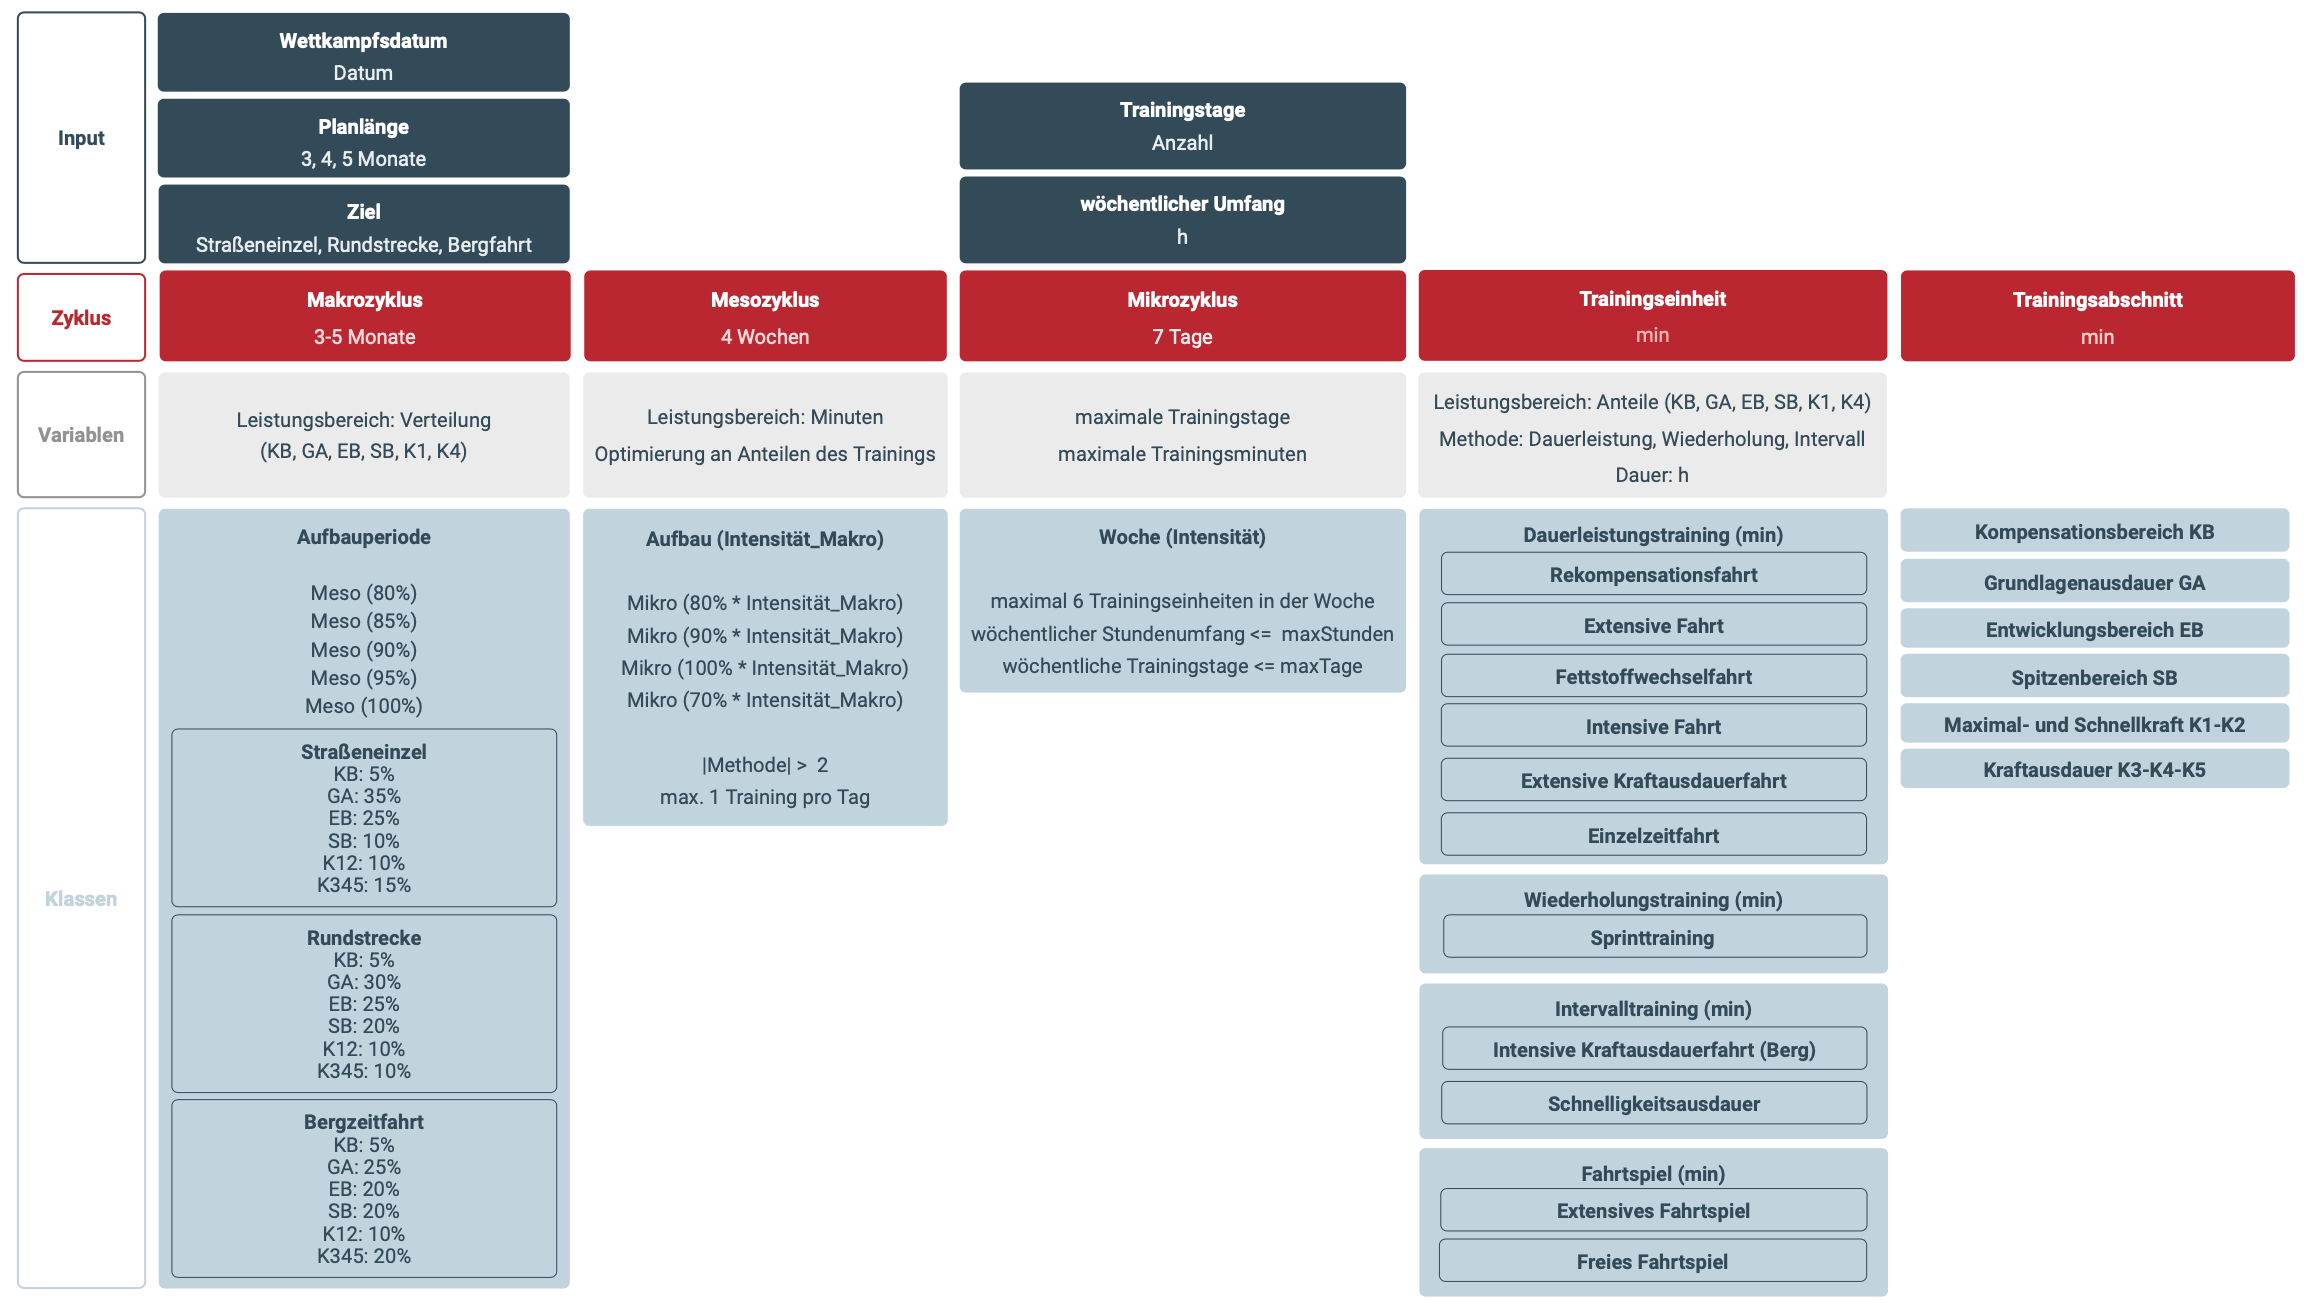
\includegraphics[width=\textwidth]{gfx/modellierung.png}
    \captionof{figure}{Schema anhand hierarchischer Zyklisierung}
    \end{minipage}
}
\newpage
\section{Mathematische Modellierung}
\label{anhang:modell}
Für jeden Tag $i \in [0, 27]$ gilt:

\begin{equation*}
    {duration}_i \mod 15 = 0
\end{equation*} 
\begin{equation*}
    r_i \mod 15 = 0, \forall r \in R
\end{equation*}
\begin{equation*}
    \sum_{r\in R} r_i = duration_i
\end{equation*}
\begin{equation*} 
    |\{method_i = m\}| \geq 2, \forall m \in M
\end{equation*} 
\begin{equation*}
    method_i = \text{PAUSE} \Leftrightarrow duration_i = 0
\end{equation*}
\begin{equation*}
    (method_i = \text{Fahrtspiel})\Rightarrow t_i = \begin{array}{c}
            (0, [\![15, 240]\!], [\![15, 240]\!], 0, 0, 0) \\ 
        \vee (0, [\![15, 300]\!], [\![15, 300]\!], [\![15, 300]\!], [\![0, 180]\!], [\![15, 180]\!])
    \end{array}
\end{equation*}
\begin{equation*}
    (method_i = \text{Dauerleistung})\Rightarrow t_i = \begin{array}{c}
            ([\![15, 180]\!], 0, 0, 0, 0, 0) \\ 
            \vee (0, [\![30, 300]\!], 0, 0, 0, 0) \\  
            \vee (0, [\![60, 300]\!], 0, 0, 0, 0) \\  
            \vee (0, [\![30, 60]\!], [\![15, 60]\!], 0, 0, 0) \\  
            \vee (0, [\![30, 60]\!], 0, 0, [\![15, 150]\!], 0) \\
            \vee (0, [\![30, 60]\!], 0, [\![15, 60]\!], 0, 0) \\  
    \end{array}
\end{equation*}
\begin{equation*}
    (method_i = \text{Intervall})\Rightarrow t_i = \begin{array}{c}
            (0, [\![30, 90]\!], 0, 0, 0, [\![15, 120]\!]) \\ 
        \vee (0, [\![60,180]\!], 0, [\![15, 45]\!], 0, 0)
    \end{array}
\end{equation*}
\begin{equation*}
    (method_i = \text{Wiederholung})\Rightarrow t_i = \begin{array}{c}
            (0, [\![15, 30]\!], 0, [\![15, 60]\!], 0, 0)
    \end{array}
\end{equation*}
Für jede Woche $w \in [0, 3]$ gilt:
\begin{equation*}
    \sum_{j=7*w}^{7*w+6} duration_j \leq maxminutes_w
\end{equation*}
\begin{equation*}
    \sum_{j=7*w}^{7*w+6}  (duration_j > 0) \leq maxdays
\end{equation*}
\begin{equation*}
    \text{minimize} \sum_{r\in R} |target_r - \sum_{i=0}^{28}r_i|
\end{equation*} 
\newpage
\section{Klassendiagramm}
\label{anhang:uml}
\begin{figure}[h]
    \begin{tikzpicture}
        \umlclass[y=11, fill=white]{Main}{
        }{
            + monitorStats() \\
            + createPlan() \\
            + createTable(i : int) \\
            + createPDF(i : int) \\}
        \umlclass[x=8, y=11, fill=white]{OutputTrainingTable}{
        }{
            + displayPlan() : void \\
        }
        \umluniassoc[arg=-table , mult2=1, pos =0.95, align=right]{Main}{OutputTrainingTable}
        \umluniassoc[arg=-plan , mult2=0..1, pos =0.77, align=right]{Main}{Macro}
        
        \umlclass[y=5, fill=white, type = abstract]{Macro}{
            - numMonth : int \\
            - maxTrainingMinutes : int \\
            - maxTrainingDays : int \\
            - compDay : LocalDate \\
            - ranges : Map<Range, Double> \\
        }{
            \umlvirt{+ setRanges()} \\
            + validateRanges()\\
            + solvePlan() \\
        }
        
        \umlclass[x=8, y=5, fill=white]{Meso}{
            - model : Model \\
            - plan : Solution \\
            - targetRanges : int[6] \\
            - targetMinutes : int[4] \\
            - name : IntVar[] \\
            - minutes : IntVar[] \\
            - method : IntVar[] \\
            - ranges : IntVar[][] \\    
            - distanceRanges : IntVar[] \\
            - overallDistance : IntVar \\

        }{
            - initializeModel() \\
            - defineConstraints() \\
            - addSessionPool(Method m, SessionPool[] p) \\
            + solveMonth() \\
            + getPlan() : Solution \\
            + getSessions() : Session[] \\
        }
        \umlclass[x=8, y=-3, fill=white]{Session}{
            - name : String \\
            - minutes : int \\
            - distribution : HashMap<Range, Integer> \\
            - day : LocalDate \\
            - method : Method \\
        }{
        }
        \umlclass[x=1, y=0, fill=white]{Strasseneinzel}{}{+ setRanges()}
        \umlclass[x=1, y=-2, fill=white]{Rundfahrt}{}{+ setRanges()}
        \umlclass[x=1, y=-4, fill=white]{Bergfahrt}{}{+ setRanges()}
        
        \umlHVinherit[anchor2=-130]{Strasseneinzel}{Macro}
        \umlHVinherit[anchor2=-130]{Rundfahrt}{Macro}
        \umlHVinherit[anchor2=-130]{Bergfahrt}{Macro}
        \umluniassoc[arg=-mesos ,  mult2=3..5, pos =0.95, align=right]{Macro}{Meso}
        \umluniassoc[arg=-sessions , mult2=28, pos =0.80, align=right]{Meso}{Session}
    \end{tikzpicture}
    \caption{Klassendiagramm der vollständigen Anwendung}
    \label{fig:uml:solver}
\end{figure}

\newpage
\section{Grafische Benutzungsoberfläche}
\rotatebox{90}{\begin{minipage}{0.9\textheight}
    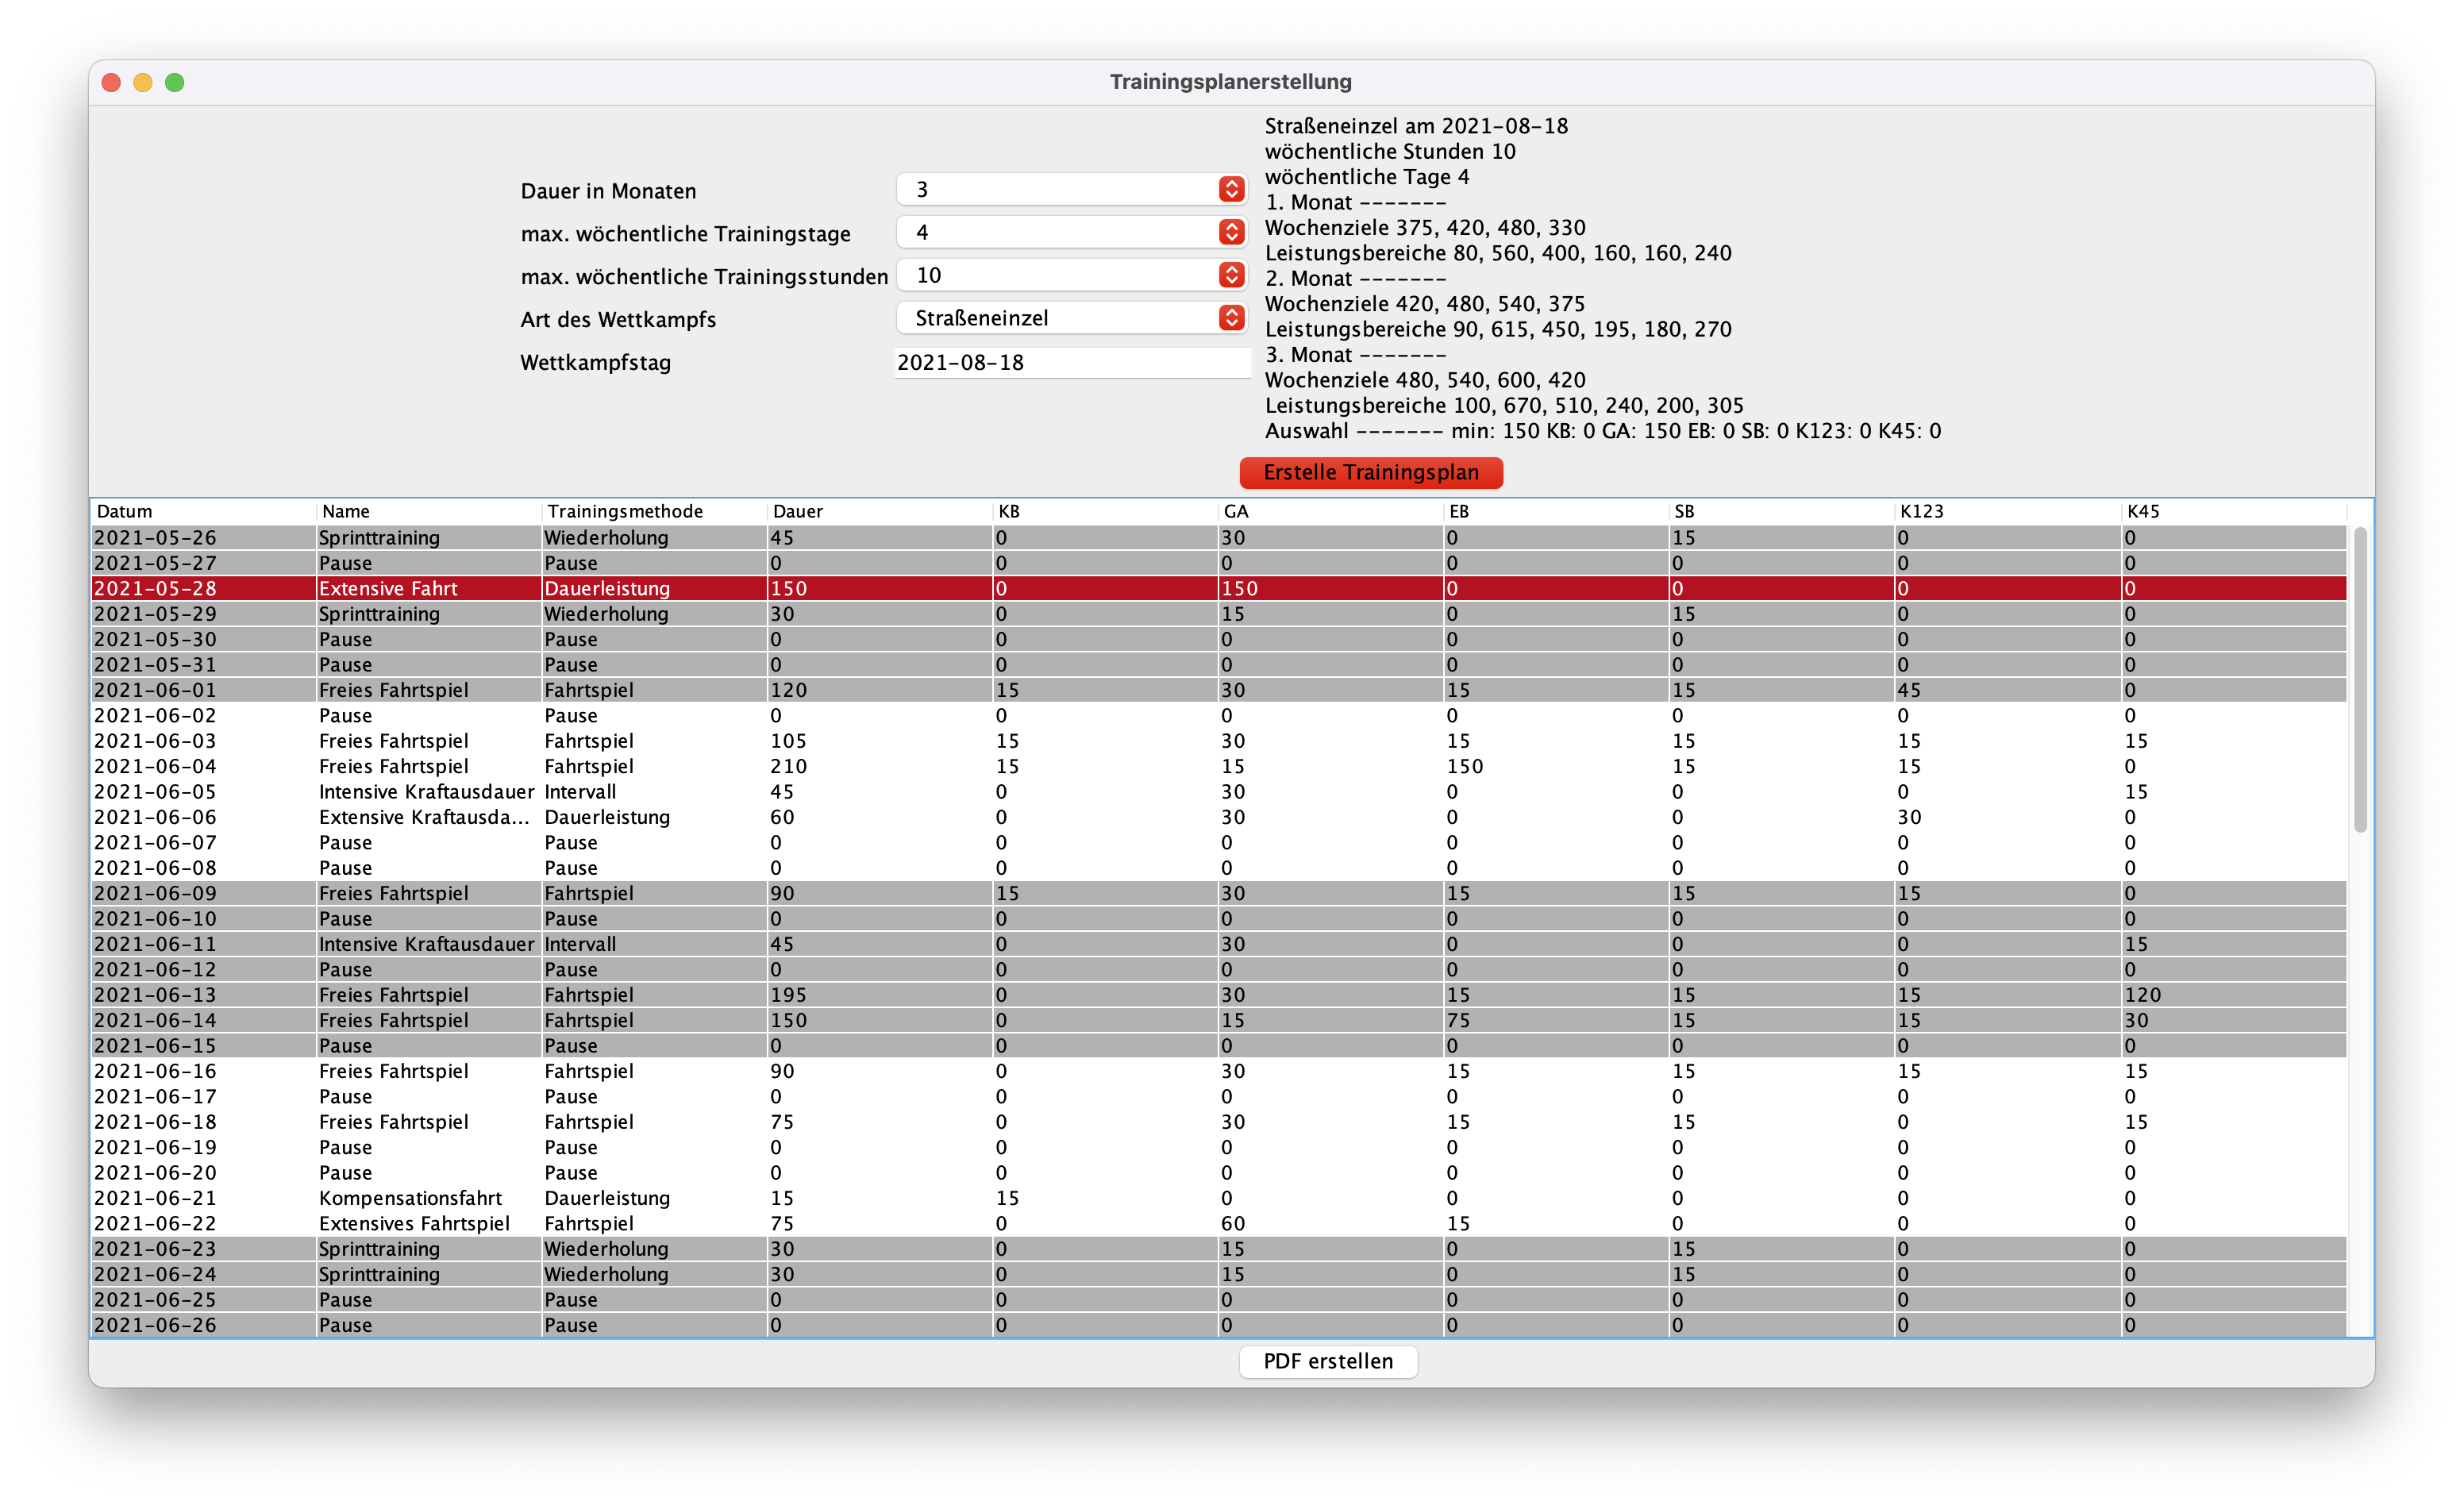
\includegraphics[width=\textwidth]{gfx/gui.png}
    \captionof{figure}{Bildschirmaufnahme der grafischen Oberfläche}
    \end{minipage}
}
\label{anhang:gui}

\newpage
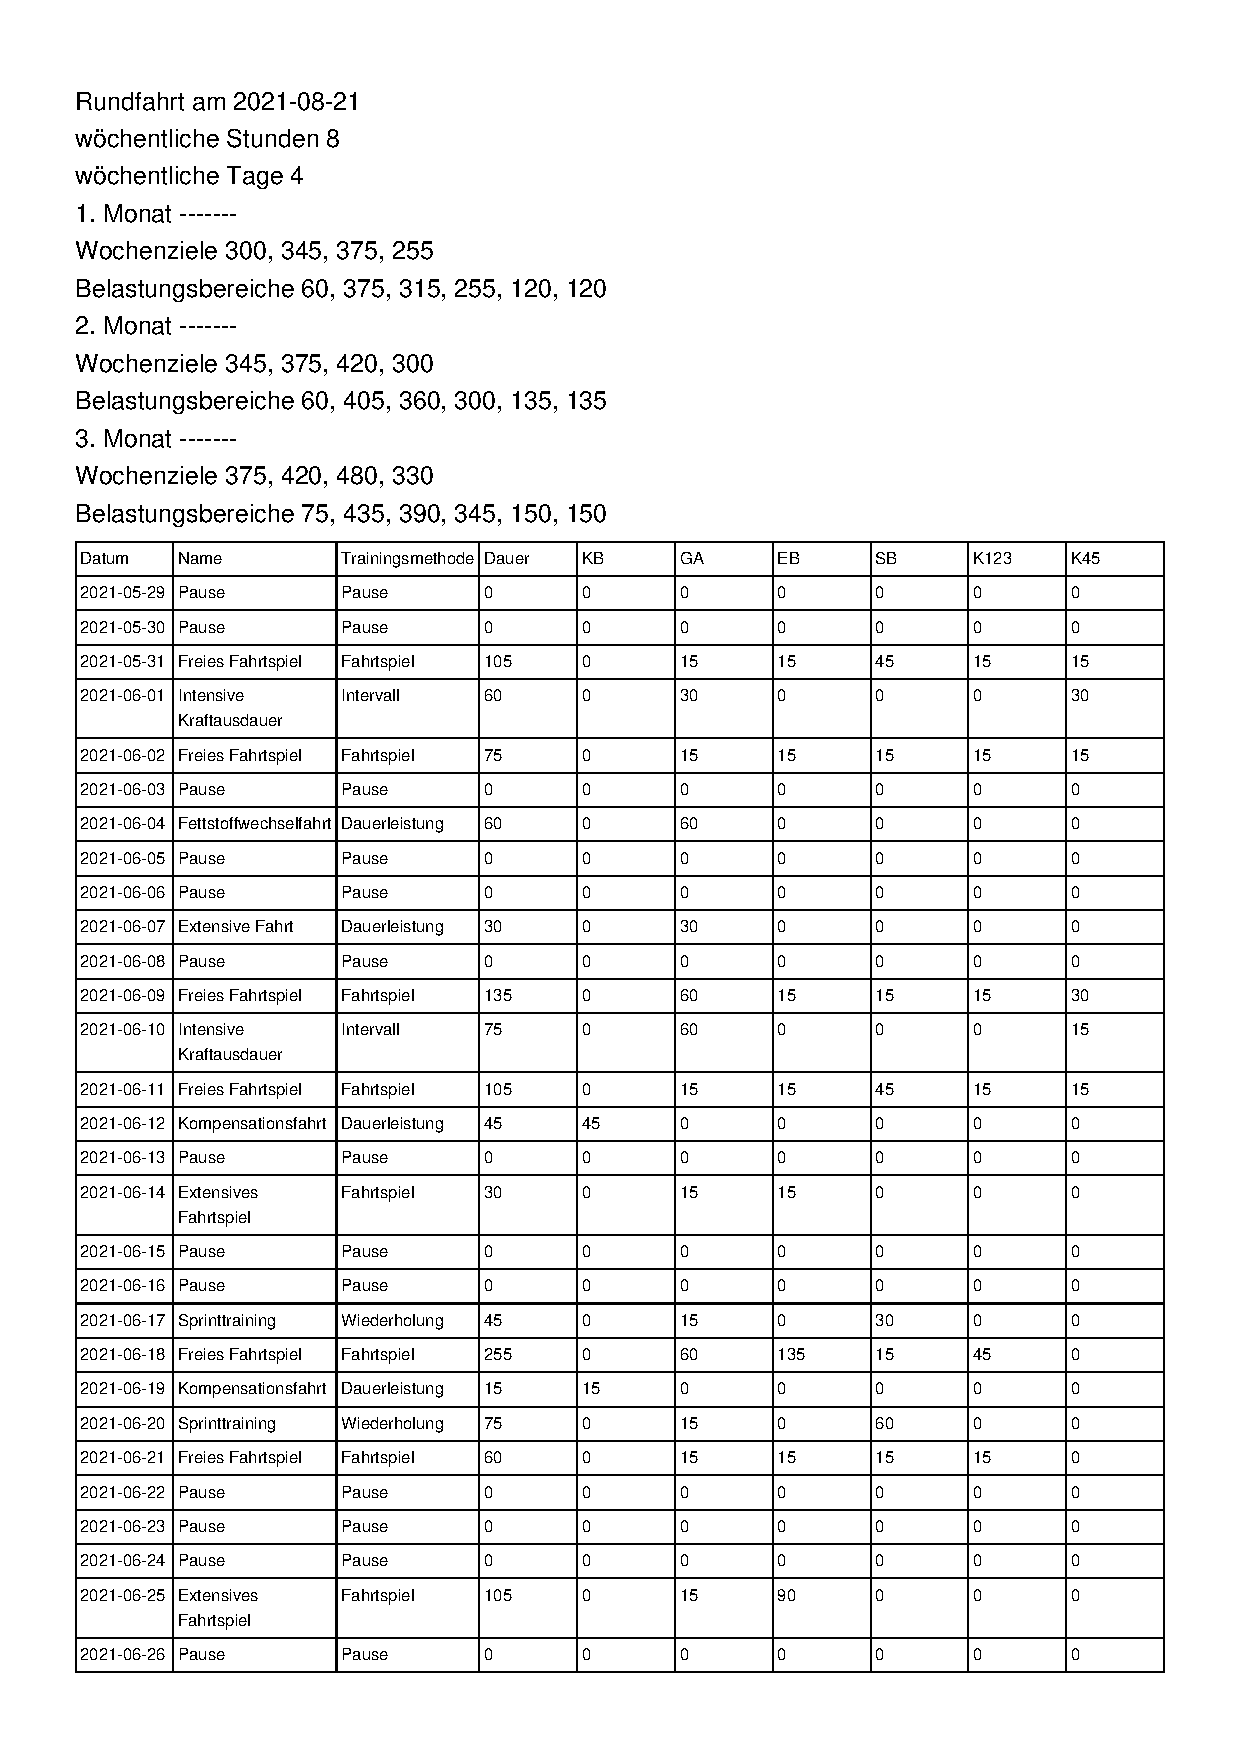
\includepdf[pages=1, scale=0.8, pagecommand=\section{Beispiel Trainingsplan}]{gfx/TimetrialCompetition_4d_8h.pdf}
\label{anhang:beispielplan}
\includepdf[pages=2-, scale=0.8]{gfx/TimetrialCompetition_4d_8h.pdf}

\newpage

\section{Schnittstelle im JSON-Format}
\label{anhang:json}
\begin{lstlisting}[language=json,firstnumber=1]
{ 
    "num_months": 3,
    "competition": "singleday",
    "sport": "racing bike",
    "competition_date": 22.02.2022,
    "sessions": [
        {
            date: 01.02.2022,
            minutes: 60,
            method: "intervall",
            name: "sprinttraining", 
            sections: [
                {
                    length: 45,
                    range: "GA"
                },
                {
                    length: 5,
                    range: "EB"
                },
                ...
            ]
        }
    ], 
}
\end{lstlisting}